\documentclass{beamer}

\usetheme{Warsaw}
\usecolortheme{seahorse}
\setbeamertemplate{navigation symbols}{}
\setbeamercolor{background canvas}{bg=}
\usepackage{beamerthemesplit}
\usepackage{pgf}
\usepackage{epsfig}
\usepackage{epstopdf}
\usepackage{graphicx}
\usepackage{slashbox}
\usepackage{url}
\usepackage{listings}
\newcommand{\IR}{\bbold R}
\def\Rset{\mathbb{R}}
\def\Zset{\mathbb{Z}}
\newcommand{\refbr}[1]{(\ref{#1})}
\newcommand{\beq}{\begin{equation}}
\newcommand{\eeq}{\end{equation}}
\newcommand{\und}[1]{\underline{#1}}

\hypersetup{
   pdftitle={Piotr Trojanek, MMAR 2007},
   pdfauthor={Piotr Trojanek, IAiIS},
   pdfborder={0 0 0}
}

\title[jPar \insertframenumber/\inserttotalframenumber]{jPar -- a simple, free and lightweight tool for parallelizing Matlab
calculations on multicores and in clusters}
\author[Andrzej Karbowski]{\textbf{Andrzej Karbowski\inst{1,2}, Marek Majchrowski\inst{1},\\
Piotr Trojanek\inst{1}, Tomasz Pokorski\inst{1},
Dawid Za{\l}uga\inst{1} }}
\institute{$^1$Institute of Control and Computation Engineering\\%
Warsaw University of Technology
\and
$^2$NASK (Research and Academic Computer Network),\\
Warsaw, Poland}


%\date{Siedlce, \today}
\date{\tiny{\emph{FedCSIS 2015 - Federated Conference on Computer Science and Information Systems,\\
{\L}\'{o}d\'{z}, Poland, 13 - 16 September, 2015
}}}

\begin{document}

\frame{\titlepage}

\frame{\tableofcontents\frametitle{The contents}}

\section{Introduction}
\begin{frame}
\frametitle{Drawbacks of Matlab Parallel  Computing
Toolbox and Distributed Computing Server}
\begin{itemize}
\item  Matlab PCT/DCS are far from stability, that is, there are
   many differences between the subsequent versions. For example, in recent versions
   there were changes concerning two commands: {\tt matlabpool} (which was replaced
   in R2013b release  by {\tt parpool} and completely removed since release R2015a) and {\tt mapreduce};
\item  if one wants to perform computations in clusters, except Matlab PCT  it is necessary to buy Matlab DCS, which is much more expensive
   and complicated in administration;
\item  universities and research laboratories usually buy Matlab
   licenses in packs; this means, that after hours in labs many licenses
   are free.
\end{itemize}
\end{frame}

\begin{frame}
\frametitle{Common drawbacks of other available parallel Matlab packages}
\begin{itemize}
\item they use use disk files for communication between
Matlab instances, what is inefficient and prone to errors.
\item depend on \emph{rsh}/\emph{ssh}
\item introduce new, complicated syntax for user to learn
\item require low-level programming knowledge (e.g. \emph{MPI})
\item they do not always work under new versions of Matlab
\end{itemize}
\end{frame}

\begin{frame}
\frametitle{Original \emph{Paralize}}
\begin{description}
 \item[Web Repository] Matlabcentral:
\url{http://www.mathworks.com/matlabcentral/}

\item[Author:] prof. Thomas Abrahamsson, Chalmers
Tekniska H$\ddot{o}$gskola, 1997;\\
\item[update]
Andrzej Karbowski, 2006\\
\end{description}
\begin{itemize}
\item [$+$] portable (implemented purely in .m scripts)
\item [$+$] easy to install and use\\
(consists of only two m-functions: {\tt paralize.m} and {\tt
serve.m} of, correspondingly, 146 and 94 lines)
\item [$-$] implements fork-join  model of parallel
computations
\item [$-$] data exchange via network filesystem
\item [$-$] servers take work by active pooling (busy waiting)
\end{itemize}
\end{frame}

\begin{frame}
\frametitle{Goals of jPar}
\begin{itemize}
\item portable (implemented in Java and .m scripts)
\item possibly small
\item easy to install and use
\item without communication via filesystem
\item without active pooling
\item can pass sparse matrices as arguments
\item function handles can be actual parameters
of parallelized functions
\end{itemize}
\end{frame}


\section{Operation details}

\begin{frame}
\frametitle{Distributing the work}
Steps:
\begin{enumerate}
\item Division of the~data
\item Passing of the data chunks together with function
      to be executed (\emph{task}) to \emph{solvers}
\item Execution of the same operation on all chunks  by slave Matlab processes (\emph{solvers})
\item Gathering the results on the~\emph{console} Matlab session (i.e. client)
\end{enumerate}
\end{frame}

\begin{frame}
\centering
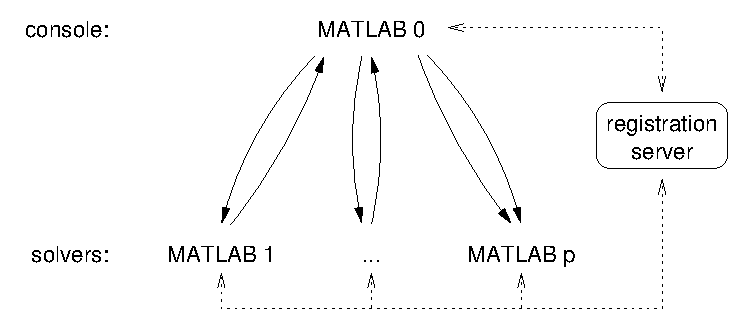
\includegraphics[width=\columnwidth]{parajava_schemat.eps}
\begin{enumerate}
\item \emph{Registration server}
\item \emph{Solvers}
\item \emph{Client}
\end{enumerate}
\end{frame}

\section{Implementation details}

\defverbatim\testcode{%
\begin{verbatim}
>> a = rand(100,100,10) + i*rand(100,100,10);}
>> [V,D] = jpar_client('eig', a);
\end{verbatim}}%

\begin{frame}[fragile]
\uncover<1->{
\frametitle{Interface between client and solvers}
\begin{itemize}
\item input data are represented as three dimensional matrices
\item job division into chunks is done by separating along the third index
\item all the remaining parameters are passed unmodified to \emph{solvers}
\end{itemize}
}
\uncover<2->{
\structure{
Example:
\testcode
}
}
\end{frame}

\defverbatim\testcodee{%
\begin{verbatim}
public class JMArray
  implements Serializable {

  private Object realpart, imagpart;
  private int dimX, dimY;
  /* ... */
}
\end{verbatim}}%

\begin{frame}[fragile]
\uncover<1->{
\frametitle{Passing numerical data between Java and Matlab}
\begin{itemize}
\item basic types are automatically converted
\item imaginary part has to be preserved
\item arrangement of arrays has to be preserved
\end{itemize}
}
\uncover<2->{
\structure{Internal representation:

\testcodee
}
}
\end{frame}

\defverbatim\testcodeee{%
\begin{verbatim}
public class JMStruct
  implements Serializable {

  private Object fields, values;
  private int dimX, dimY;
  /* ... */
}
\end{verbatim}}%

\begin{frame}[fragile]
\uncover<1->{
\frametitle{Handling mixed data}
\begin{itemize}
\item strings
\item structures of optimization options (e.g. {\itshape fmincon})
\item recursive data conversion
\end{itemize}
}
\uncover<2->{
\structure{Internal representation:

\testcodeee
}
}
\end{frame}
\begin{frame}[fragile]
\section{Installation and using jPar}
\frametitle{The installation and starting jPar}
It is very simple:
\begin{enumerate}
\item Copy file .java.policy to home directory (in Windows use
   " Documents and Settings$\setminus$Username" directory) or use "install.bat" (Windows)
   or "sh ./install.sh" (Unix) on every node, where you want to run
   jPar client or solver
\item Run one instance of paralize server using "jpar\_server.bat" (Windows)
   or "sh ./jpar\_server.sh" (Unix) on node, where you want to run paralize
   clients
\item Start Matlab sessions in the directory which contains
   jPar files
\item Start solvers from Matlab session in jPar directory
   using:\\

   \textcolor{blue}{\tt >> jpar\_solver('<hostname>');}

   where {\tt <hostname>} is the name of host where jPar server is running
   (default to localhost)\\
\end{enumerate}
\end{frame}
\begin{frame}
\frametitle{Starting application}
A distributed application is started with:\\
\vskip 0.2cm
\textcolor{blue}{\tt >> [<output>] =...}\\
 \hspace{0.5cm} \textcolor{blue}{\tt jpar\_client(<name\_of\_function>, <parameters>)}  \\
\vskip 0.2cm
After the work is done, the user should kill solvers :\\
\vskip 0.2cm
\textcolor{blue}   {\tt >> jpar\_client('kill');}\\
\vskip 0.2cm
To see free solvers one may use the command:\\
\vskip 0.2cm
 \textcolor{blue}   {\tt >> jpar\_client('hosts');}

\end{frame}
\section{Case-study results}

\begin{frame}
\frametitle{General separable optimization problem}
\beq
\min_{x \in X} \sum_{i=1}^p f_i(x_i)
\label{zad.sep.wj}
\eeq
\beq
\sum_{i=1}^p g_{ji}(x_i) \leq M_j, \;\;\;  j=1,\ldots,m
\eeq
\beq
x =(x_1,x_2,\ldots,x_p) \in
X=X_1 \times X_2 \times \ldots X_p
\eeq
\beq X_i \subseteq \Rset^{n_i},\;\;\, n=\sum_{i=1}^p n_i
\label{zad.sep.kon}
\eeq
where all  functions $f_i$ are strictly convex, $g_{ji}$ - convex.
\end{frame}

\begin{frame}
\frametitle{Dual (price) method}
Decomposition of the Lagrangian:
\[
L_D(\lambda) = \min_{x \in X} \left[ L(x,\lambda) =
\sum_{i=1}^p f_i(x_i) + \sum_{j=1}^m \lambda_j \cdot \left( \sum_{i=1}^p g_{ji}(x_i) -
M_j \right) \right]
 =
\]
\[
= \min_{x_i \in
X_i , i=1,\ldots,p} \left[ \sum_{i=1}^p \left(f_i(x_i) +
\sum_{j=1}^m \lambda_j  g_{ji}(x_i) \right) - \sum_{j=1}^m \lambda_j
M_j \right] =
\]
\beq
=\sum_{i=1}^p \min_{x_i \in X_i} \left( f_i(x_i) +
\sum_{j=1}^m \lambda_j  g_{ji}(x_i) \right) - \sum_{j=1}^m \lambda_j
M_j
\label{f.dualna}
\eeq
\end{frame}

\begin{frame}
\frametitle{Master-slave approach}
\begin{enumerate}
\item $p$ Local problems; the $i$-th:
\beq
\min_{x_i \in X_i} \left[ L_i(x_i,\lambda)=f_i(x_i) + \sum_{j=1}^m \lambda_j  g_{ji}(x_i)\right]
\eeq
\hspace{1cm}$x_i(\lambda)$  is its solution.
\item Coordination problem:
\beq
\max_{\lambda \geq 0} \left[ L_D(\lambda)= \sum_{i=1}^p L_i(x_i(\lambda),\lambda)
           - \sum_{j=1}^m   \lambda_j M_j \right]
\eeq
\end{enumerate}
\end{frame}

\begin{frame}
\frametitle{Powell20 test problem}
\beq
    \min_{x} 0.5 \cdot ( x_1^2+x_2^2+....+x_n^2 )
\eeq
\beq
                 x_{k+1}-x_{k} \geq -0.5+(-1)^k\cdot k; \;\; k=1,\ldots,n-1
\eeq
\beq
                  x_1-x_n \geq n-0.5
\eeq
\end{frame}
\begin{frame}[fragile]
\frametitle{The parallelization}
It was necessary ONLY to replace the lines:
\begin{verbatim}
for i=1:p
  [xi(:,1,i),fi(1,1,i)]=...
       pow20_pm_loct(xloc(:,1,i),lambda,ni,p,options_k);
end
\end{verbatim}
with the line
\begin{verbatim}
  [xi,fi]=jpar_client('pow20_pm_loct',...
                            xloc,lambda,ni,p,options_k);
\end{verbatim}
\end{frame}

\begin{frame}
\frametitle{The speed-up of parallelization and \textcolor{red}{decomposition}}
\centering
\includegraphics[height=6.5cm]{fig1}
\end{frame}
\begin{frame}
\frametitle{The speed-up of parallelization and \textcolor{red}{decomposition}}
\centering
\includegraphics[height=6.5cm]{fig2}
\end{frame}
\begin{frame}
\frametitle{The speed-up of parallelization and \textcolor{red}{decomposition}}
\centering
\includegraphics[height=6.5cm]{fig3}
\end{frame}
\begin{frame}
\frametitle{The speed-up of parallelization and \textcolor{red}{decomposition}}
\centering
\includegraphics[height=6.5cm]{fig4}
\end{frame}
\begin{frame}
\frametitle{The speed-up of parallelization and \textcolor{red}{decomposition}}
\centering
\includegraphics[height=6.5cm]{fig5}
\end{frame}

\section{Conclusions}

\begin{frame}[allowframebreaks,fragile]
\frametitle{Conclusions}
\begin{enumerate}
\item The jPar is:
\begin{itemize}
\item relatively small (about 800 lines of Java code and 400 lines of Matlab code)
\item simple in installation
    \item simple in use (the changes in sequential code are very small)
\item reliable (there are no errors caused by disk transmissions)
\item heterogenous (Linux, Windows, OS X)
\item interoperable between various Matlab and Java versions
 \item open and free (can be downloaded from the MatlabCentral page
     \url{http://www.mathworks.com/matlabcentral/fileexchange/50797} )
\end{itemize}
\newpage
\item Avoiding active
polling it does not waste the energy, network resources and does
not block the cores waiting for tasks
\item The problems that may be solved should have fork-join structure, without communication between instances)
  \end{enumerate}
\end{frame}
\begin{frame}
\frametitle{Successful application of jPar abroad}
A beta version of {\emph jPar}  in:
\begin{enumerate}
\item MEIGO system: \\
{\em J.A. Egea, D. Henriques, T. Cokelaer, A.F. Villaverde, A. MacNamara, D.-P. Danciu, J.R. Banga and J. Saez-Rodriguez, ``MEIGO: an open-source software suite based on metaheuristics for global optimization in systems biology and bioinformatics", BMC Bioinformatics, vol. 15,  2014.}
\item CeSS system:\\
{\em D.R. Penasa, P. Gonz\'{a}lez , J.A. Egea, J.R. Banga and R. Doallo,
``Parallel Metaheuristics in Computational Biology: An Asynchronous Cooperative Enhanced Scatter Search Method", Procedia Computer Science, vol. 51, 2015, pp.  630--639}
\end{enumerate}
in Department of Applied Mathematics and Statistics, Universidad Politécnica de Cartagena,
(Bio)Process Engineering Group, Spanish National Research Council,
European Molecular Biology Laboratory, Cambridge,
Instituto de Investigaciones Marinas
\end{frame}
\end{document}
